\pdfminorversion=7
\documentclass[oneside,openany]{amsdtx}
\usepackage[margin=.75in]{geometry}
\usepackage{graphicx,float,amsmath,amssymb,booktabs,array,enumitem}
\usepackage[T1]{fontenc}\usepackage[utf8]{inputenc}\usepackage[english]{babel}
\usepackage{lmodern,siunitx,xcolor}\usepackage[colorlinks=true,allcolors=blue,hyperindex=false]{hyperref}
\newcolumntype{L}[1]{>{\raggedright\arraybackslash}p{#1}}
\title{\sc Thermochemical Simulation of the Iris Phenolic Liners\\\large Setup and Accepted Results}
\author{\sc MIT Rocket Team --- Solid Propulsion Simulations}
\date{November 03, 2026 at 22:33 EST}
\begin{document}\maketitle
\begin{center}
\includegraphics[height=1.1cm]{logos/rtlogo.pdf}\hspace{2cm}
\includegraphics[height=.65cm]{logos/ansys.png}\end{center}
\begin{center}\fbox{\begin{minipage}{.93\textwidth}\small
\textbf{Exploratory study.} Four configurations are considered: sustainer and booster, each with an aluminium or carbon-fibre composite casing. Heat flux, firing duration, grain port and measured recession are unavailable. The user authorized explicit surrogate inputs and sensitivity studies. This report separates native numerical checks from physical calibration. A pilot is not a demonstrated motor lifetime.
\end{minipage}}\end{center}
\tableofcontents
\clearpage
\section{Purpose and definition of burnthrough}
The primary event is exhaustion of the continuous phenolic barrier, leaving the casing exposed in this two-layer geometry. Pyrolysis conversion alone is not this event: char remains solid and can continue insulating. We report remaining physical thickness, actual geometric recession, conversion depth and casing temperatures separately. Burnthrough is bracketed by the last accepted intact state and first exhausted state.

The calculation represents an initially intact, locally uniform wall. Cracks, joints, debonding, char spallation and particle erosion are not resolved. Material-temperature flags indicate the scope of surrogate properties, not certified pressure-casing failure. If the event is absent, the result is ``not reached through the simulated exposure,'' with residual thickness, rather than an extrapolated lifetime.

\section{Geometry and discretization}
The supplied propellant radii are provisionally used as liner inner radii. No unreported gap or adhesive layer is inserted. The user requested short axial and sector slices with about twenty radial cells per material. Each exchanged STEP contains exactly two solids and is reimported independently to verify volumes and dimensions.
\begin{table}[H]\centering\small
\begin{tabular}{lrrrr}\toprule
Motor & Bore radius & Phenolic & Case & Outside radius\\
 & \multicolumn{4}{c}{Dimensions in millimetres}\\\midrule
Sustainer & 39.6875 & 4.7625 & 3.1750 & 47.6250\\
Booster & 65.0875 & 6.3500 & 4.7625 & 76.2000\\\bottomrule
\end{tabular}\end{table}
Al and CF versions share the dimensions within each motor. The initial domain is \SI{0.5}{mm} long and \(0.5^\circ\) wide, with 2 axial and 2 angular divisions. Twenty radial cells in each material give 160 SOLID278 elements and 369 nodes. The axis is global Y. Lateral and axial faces are adiabatic under the uniform-wall assumption. Integrated mass/power scales by 720 to a full ring of the same short length; temperatures and recession do not scale.
\begin{figure}[H]\centering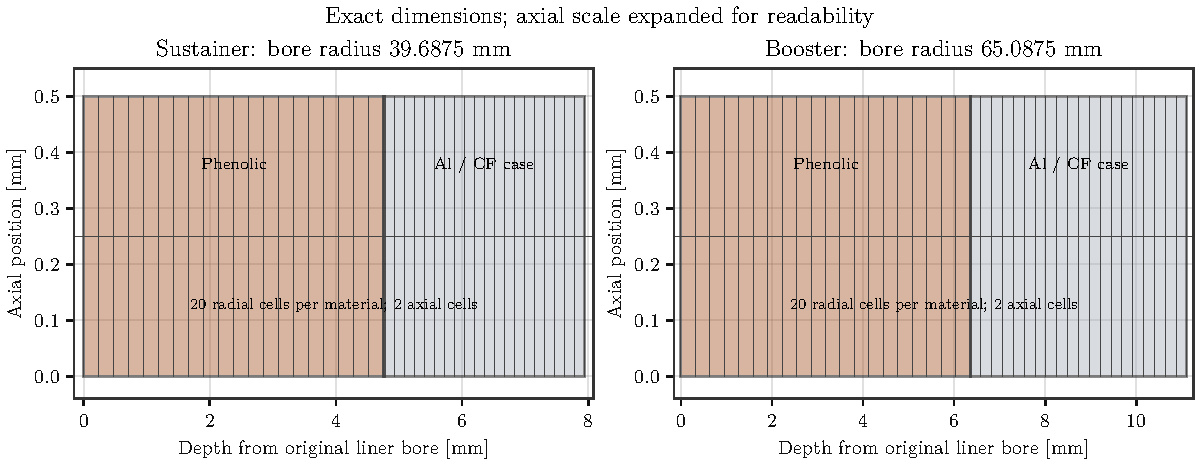
\includegraphics[width=\textwidth]{../analysis/geometry_mesh.pdf}\caption{Radial/axial mesh projections. The angular direction has two divisions; axial scale is expanded. These are setup diagrams, not solved contours.}\end{figure}
STEP is the exchange geometry. The native structured mesh is generated deterministically from the same dimensions; it is not an automatic mesh imported from STEP. The initial 20-cell phenolic pitches are 0.238125 mm and 0.3175 mm. Comparisons at 40 and 80 radial cells will assess thermal gradients, cell-removal quantization and retained partial-cell thermal storage. Additional refinement must be justified by the results.

\section{Materials and thermal environment}
\subsection{Phenolic and aluminium inherited from the earlier study}
The reference virgin and char densities are 1250 and \SI{600}{kg.m^{-3}}. The inherited single-step kinetics use \(A=\SI{333}{s^{-1}}\), \(E_a=\SI{64081}{J.mol^{-1}}\), order one, and an endothermic pyrolysis term of \SI{418}{kJ.kg^{-1}}. Thermal tables vary with temperature. Their applicability to the manufactured Iris liner is uncalibrated. Aluminium initially uses \(\rho=2700\), \(k=167\) and \(c_p=896\) in SI units; the exact alloy is unspecified.
\begin{figure}[H]\centering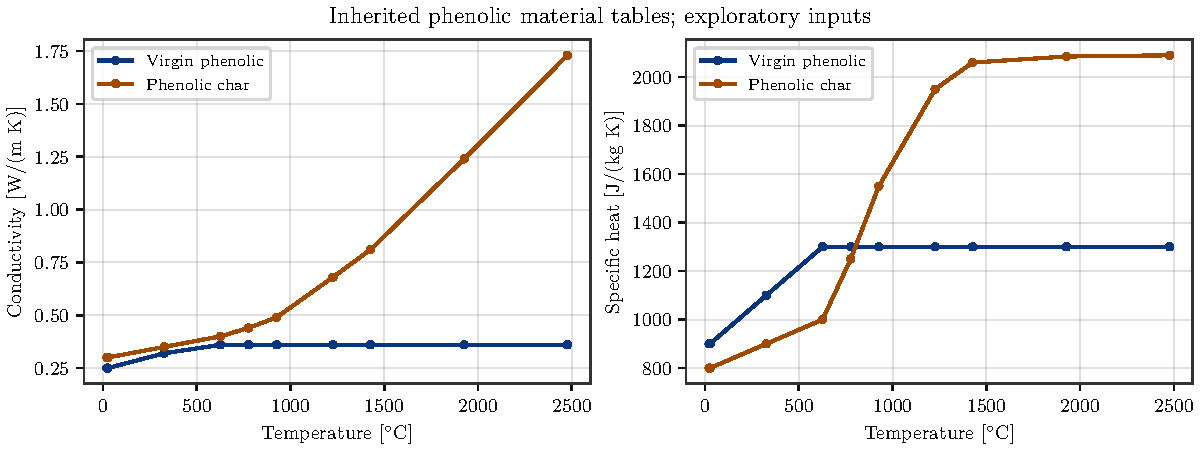
\includegraphics[width=\textwidth]{../analysis/phenolic_properties.pdf}\caption{Inherited input tables. Lines interpolate prescribed material data and are not experimental measurements made for Iris.}\end{figure}
\subsection{Carbon fibre surrogate}
The user's ACP fin tutorial supplies \(\rho=\SI{1451}{kg.m^{-3}}\), elastic and thermal-expansion data, but no CF conductivity or heat capacity. Its G10 thermal values are not used as CF properties. The initial woven-laminate surrogate has radial conductivity \SI{0.55}{W.m^{-1}.K^{-1}} and equal tangential/axial conductivities \SI{2.5}{W.m^{-1}.K^{-1}}, within the woven-composite ranges reported by Joven and colleagues~\cite{woven}. Local material frames follow the cylinder.

For heat capacity, use the separately identified T700/M21 surrogate \(c_p=2.8773T+687.31\), with Celsius temperature and SI heat-capacity units~\cite{fire}. Clamp this input above \SI{200}{\degreeCelsius}; high-temperature predictions then have a flagged material approximation. The density, conductivity and heat capacity come from different references and do not constitute a measured property set for the user's casing. A \SI{150}{\degreeCelsius} CF flag and \SI{300}{\degreeCelsius} Al flag track provisional property scope, not structural failure. NASA's alternative carbon-epoxy data provide another sensitivity reference~\cite{nasa}.

\subsection{Imposed exposure}
The initial gas-side assumption is \(T_g=\SI{2504}{K}\), unblown \(h_0=\SI{1000}{W.m^{-2}.K^{-1}}\), and nominal pressure 800 psi, following the earlier study and the user's pressure estimate. Pressure is interpreted as absolute in the char-law closure. Initial and external ambient temperature is \SI{22}{\degreeCelsius}; external convection is \SI{8}{W.m^{-2}.K^{-1}} and emissivity is 0.25. The initial hot-radiation emissivity is zero, with separate radiation sensitivity scenarios.

The liner is assumed exposed from the start of imposed heating. The actual grain shielding and local exposure history are unknown. Begin with native pilots, a 7 s comparison baseline, hypothetical 7/20/60 s pulses plus cooling, and a separate continuous-exposure branch. None of these pulse lengths is an inferred motor burn duration. Vary heat-transfer coefficient, radiation, material properties, pressure and char-consumption parameters before reporting an uncertainty envelope.

\subsection{Supplied reaction and inventory envelope}
The user's reaction is atom-balanced:
\[3\mathrm{NH_4ClO_4}+3\mathrm{Al}\longrightarrow\mathrm{Al_2O_3}+\mathrm{AlCl_3}+3\mathrm{NO}+6\mathrm{H_2O}.\]
Its reactant mass bookkeeping is approximately 81.32 percent ammonium perchlorate and 18.68 percent aluminium. With constituent densities of 1950 and \SI{2700}{kg.m^{-3}}, an ideal additive-volume binary mixture would have density \SI{2056.7}{kg.m^{-3}}. The AP density is a published material value~\cite{ap}; the binary mixture is an explicit assumption, not a measured propellant formulation.
\begin{table}[H]\centering\small
\begin{tabular}{lrrr}\toprule
Motor & Volume at 1 m [litres] & Full-cylinder mass [kg] & 0.75--1.25 m range [kg]\\\midrule
Sustainer & 4.948 & 10.18 & 7.63--12.72\\
Booster & 13.309 & 27.37 & 20.53--34.22\\\bottomrule
\end{tabular}\end{table}
These are full-cylinder envelope values with no port, binder or voids. Actual mass scales with occupied volume fraction and actual bulk density. The stoichiometric product list is not an equilibrium combustion calculation, and this inventory cannot establish burn duration, wall heat flux or char kinetics. The inherited gas temperature remains an imposed scenario. No full-length fuel cylinder is meshed.

\section{Thermochemical physics and solver}
The phenolic thermal law solves conduction with temperature/conversion-dependent properties, endothermic pyrolysis and gas sensible cooling. The reaction state follows
\[\dot\alpha=A\exp[-E_a/(RT)](1-\alpha),\qquad 0\leq\alpha\leq1.\]
The compiled UserMatTh routine integrates conversion analytically at increment midpoint temperature and requests a smaller solver increment when conversion changes too much. The gas source follows the virgin-to-char density loss. A surface blowing correction reduces convection as gas leaves the solid. Pore pressure and Darcy transport are not resolved.

A separate effective char-consumption law combines kinetic and mass-transfer limits and available surface energy. The inherited effective removal cost is \SI{35}{MJ.kg^{-1}}. This is an exploratory closure, not a calibrated oxidation mechanism. A row is scheduled for removal only after residual solid mass falls below 0.1 percent of its initial virgin mass. Hot-face loads move to the next live row. Consumed char remains in the live finite-element thermal representation until row removal; its numerical influence must be bounded through refinement or a revised partial-cell treatment.

MAPDL 2026 R1.02 runs natively in Windows through the Parallels VM, using the previous x64 material DLL and the installed Python coupling controller. The initial tiny models use one process. At every coupling step, the controller checks exported time and live element identity, gas/char/solid mass, thermal energy and the actual applied hot-face power before accepting an atomic checkpoint. Native face heat rates are used, with independent reconstruction of user-material energy sinks where the native aggregate channels omit them.

The initial gates are mass residual at most \(10^{-6}\) of initial liner mass, step energy residual at most 5 percent, and hot-load error at most 2 percent. These numerical gates do not validate the material law. Comparison of mesh and coupling steps targets less than 5 percent change in event time, with event brackets and temperatures reported explicitly.

The corrected pilot exporter retrieves only defined live-material ranges. The earlier three undefined-SVAR warnings per step were removed without changing physical equations. The native user-material solve retains the standard warning that the Ansys-supplied USERCK routine is used; its banner separately confirms a user-defined thermal material. This known warning is recorded, not silently counted as zero warnings.

\section{Execution and storage controls}
The running VM has 14 virtual CPUs and approximately 112 GiB RAM. The repository is accessible through a dedicated I: mapping. A native no-solve probe completed with a successful license checkout and zero warnings/errors. Each case receives a separate sealed runtime; unchanged source hashes and expected inventories are checked before launching.

The user's storage floors are 400 GB decimal free on the Mac disk and 10 GB free on Windows C:. A host watcher checks the Mac every five seconds and the guest disk about every thirty seconds. The controller also requires a fresh storage heartbeat. On a threshold crossing, new work stops, a stop latch is written and the active solver is asked to terminate cleanly. Interrupted states are not published as accepted data.

Native results/restarts remain in ignored storage. Major setup and report milestones are pushed to GitHub after verification; staged files and new Git objects at or above 100 MB are rejected. Reports freeze accepted state indices and source hashes. Recovery preserves the failed run and matches native restart state with controller state before continuation.

\section{Accepted results at this edition}
This snapshot was frozen at November 03, 2026 at 22:33 EST. The table includes only accepted native states. A completed short pilot establishes execution of the coupled code, not convergence of lifetime. Larger temperatures or longer exposure curves will appear only when corresponding native states are accepted.
\begin{table}[H]\centering\scriptsize
\begin{tabular}{lrrrr}\toprule
Run & Time [s] & Hot face [$^\circ$C] & Remaining [mm] & Energy error [\%]\\\midrule
booster\_al\_pilot2 & 0.1000 & 680.70 & 6.35000 & 0.0517 \\
booster\_cf\_pilot2 & 0.1000 & 680.70 & 6.35000 & 0.0517 \\
sustainer\_al\_pilot2 & 0.1000 & 740.56 & 4.76250 & 0.0567 \\
sustainer\_cf\_pilot2 & 0.1000 & 740.56 & 4.76250 & 0.0567 \\
\bottomrule\end{tabular}\end{table}
\begin{figure}[H]\centering 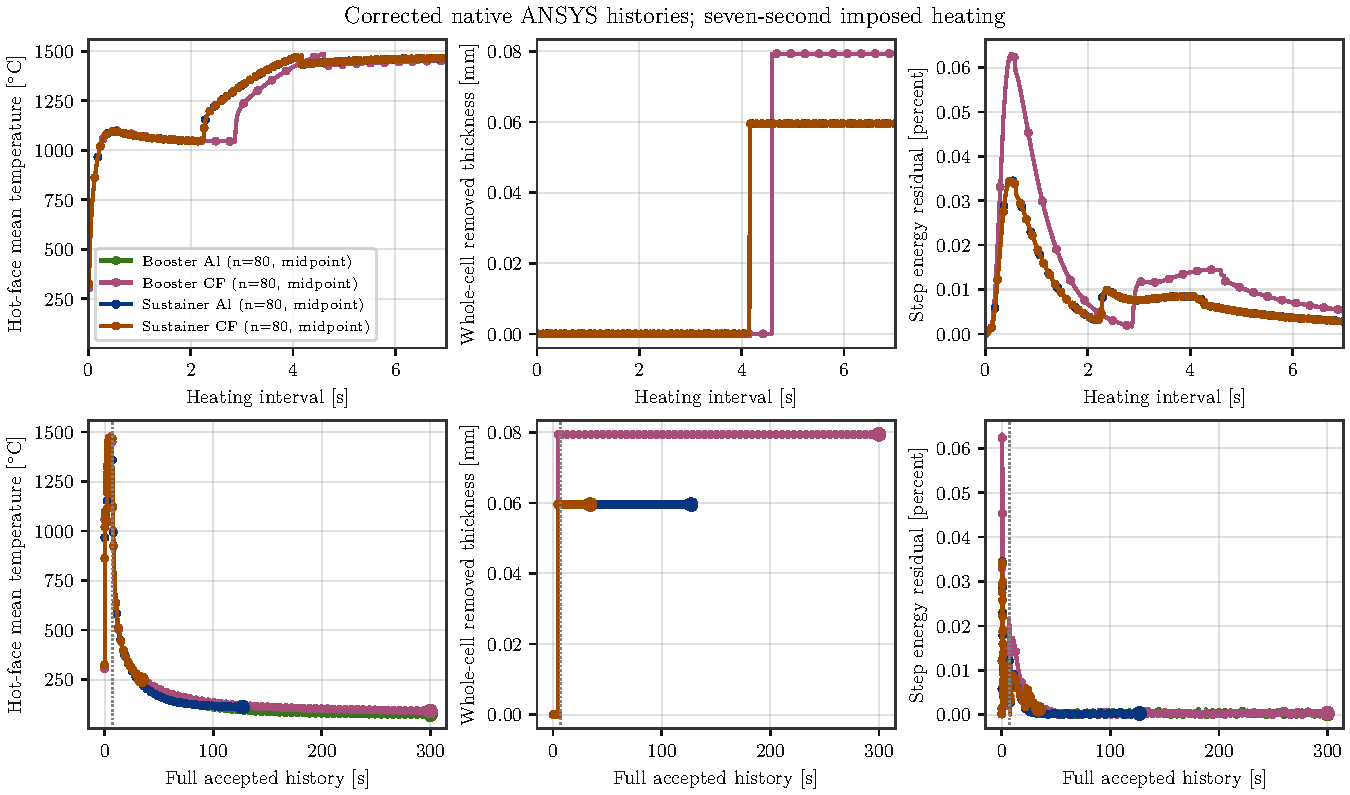
\includegraphics[width=\textwidth]{../analysis/accepted_histories.pdf} \caption{Accepted native histories. No extrapolated future states are included.}\end{figure}

\section{Outstanding verification and next results}
The four pilots are complete. Compare the independent radial model, exercise row removal and checkpoint restart, then run baseline and convergence cases. Report physical recession separately from the 98 percent pyrolysis front. Check first/last row load transfer and quantify the partial-cell approximation. Refine only when needed; the user requested small, economical meshes.

The eventual comparison will give a burnthrough bracket or an exposure-duration lower bound for each configuration, minimum remaining thickness, peak casing temperatures and their times, and sensitivity to uncertain inputs. Any entry leaving the material evidence range will remain explicitly qualified. The study cannot establish real motor lifetime without a supported wall-exposure history and recession calibration.

\begin{thebibliography}{9}
\bibitem{prior} MIT Rocket Team, \emph{Thermochemical Simulation v0: Interim Results for the New Phenolic Liner}, September 26, 2026; accompanying versioned configuration, UserMatTh source and controller in this repository.
\bibitem{acp} M. Nichitiu and C. Casebolt, \emph{ANSYS Composite Analysis for Characterization of the Project Aurora Fin Can}, user-supplied tutorial, especially pp. 3--5.
\bibitem{woven} R. Joven et al., \emph{Thermal properties of carbon fiber-epoxy composites with different fabric weaves}, 2011. \url{https://www.researchgate.net/publication/288102626}.
\bibitem{fire} P. Tranchard et al., \emph{Modelling Behaviour of a Carbon Epoxy Composite Exposed to Fire: Part I}, Materials 10(5), 494, 2017, Table 5. \url{https://doi.org/10.3390/ma10050494}.
\bibitem{nasa} M. Pauken, \emph{Simplified Plume and Aerothermal Heating Analysis for LDSD}, TFAWS 2012. \url{https://tfaws.nasa.gov/TFAWS12/Proceedings/TFAWS2012-AE-002.pdf}.
\bibitem{ap} Sigma-Aldrich, ammonium perchlorate product 455822, density \SI{1.95}{g.cm^{-3}} at \SI{25}{\degreeCelsius}. \url{https://www.sigmaaldrich.com/US/en/product/aldrich/455822}.
\end{thebibliography}
\end{document}
